\documentclass[titlepage, 11pt, reqno]{article}    % use "amsart" instead of "article" for AMSLaTeX format
\usepackage{my_packages}
\usepackage{tikz_packages}
\usepackage[american,siunitx]{circuitikz}
\usepackage{pgfplots}
\pgfplotsset{compat=1.14}
\usepackage[explicit]{titlesec}

% change the formatting for a section (which we're treating as a problem)
\titleformat{\section}[runin]{\normalfont\bfseries}{}{0em}{#1\ \thesection}
\crefformat{section}{problem #2#1#3}
\Crefformat{section}{Problem #2#1#3}


\begin{document}
\begin{titlepage}
    \centering
    \vspace{1cm}
    {\Large Spring 2017 MAE3134: Final Exam\par }
    \vspace{3cm}
    {11 May 2017\par}
    \vspace{1cm}
    \textbf{Resources allowed}: Open notes/book, calculator, ruler. 
    No computers or mobile devices.

    \vspace{1cm}
    {Name: \underline{\hspace{5cm}} \hspace{2cm} GWID:\underline{\hspace{5cm}}\par}
    \vspace{3cm}

    \begin{tabular}{|l|l|l|l|l|l|l|l|l|}
        \hline
        Prob. 1 & Prob. 2 & Prob. 3 & Prob. 4 & Prob. 5 & Prob. 6 & Prob. 7 & Prob. 8 & Total \\
        \hline
        & & & & & & & &\\[4ex]
        \hline
    \end{tabular}
    \vfill
\end{titlepage}
\section{Problem}\label{prob:sys_response_to_poles}
Elon Musk, CEO of SpaceX and Tesla Motors, has a background in physics but unfortunately has never passed a Linear Dynamics course. 
His newest space vehicle must satisfy the following second order time response specifications for a unit step input:
\begin{itemize}
    \item Percent Overshoot must be less than \(5 \%\),
    \item Rise time less than \SI{1}{\second},
    \item Settling Time less than \SI{5}{\second}.
\end{itemize}
Elon needs your help to choose a set of poles which will satisfy the specifications and save humanity from impending disaster.
\begin{enumerate}
    \item On the s-plane, or complex plane, map out the acceptable regions where you could locate poles and meet the requirements. 
    \item Label the specifications lines and show your work.
    \item Choose a set of poles that will meet the requirements.
\end{enumerate}

\begin{figure*}[htbp]
\centering
\begin{scaletikzpicturetowidth}{\textwidth}
    \begin{tikzpicture}[scale=\tikzscale]
        \draw[help lines, color=gray!30, dashed] (-8, -5) grid (8, 5);
        \draw[->, ultra thick] (-8, 0)--(8, 0) node[right]{Real};
        \draw[->, ultra thick] (0, -5)--(0, 5) node[above]{Imag};
    \end{tikzpicture}
\end{scaletikzpicturetowidth}
\end{figure*}

\newpage
\thispagestyle{plain}
\mbox{}

\newpage
\section{Problem}\label{prob:bode_response_analysis}

The frequency response of two systems are shown in~\cref{fig:prob1_bode}.
Using the plots, circle the correct descriptions:
\begin{figure}[htbp]
    \centering
    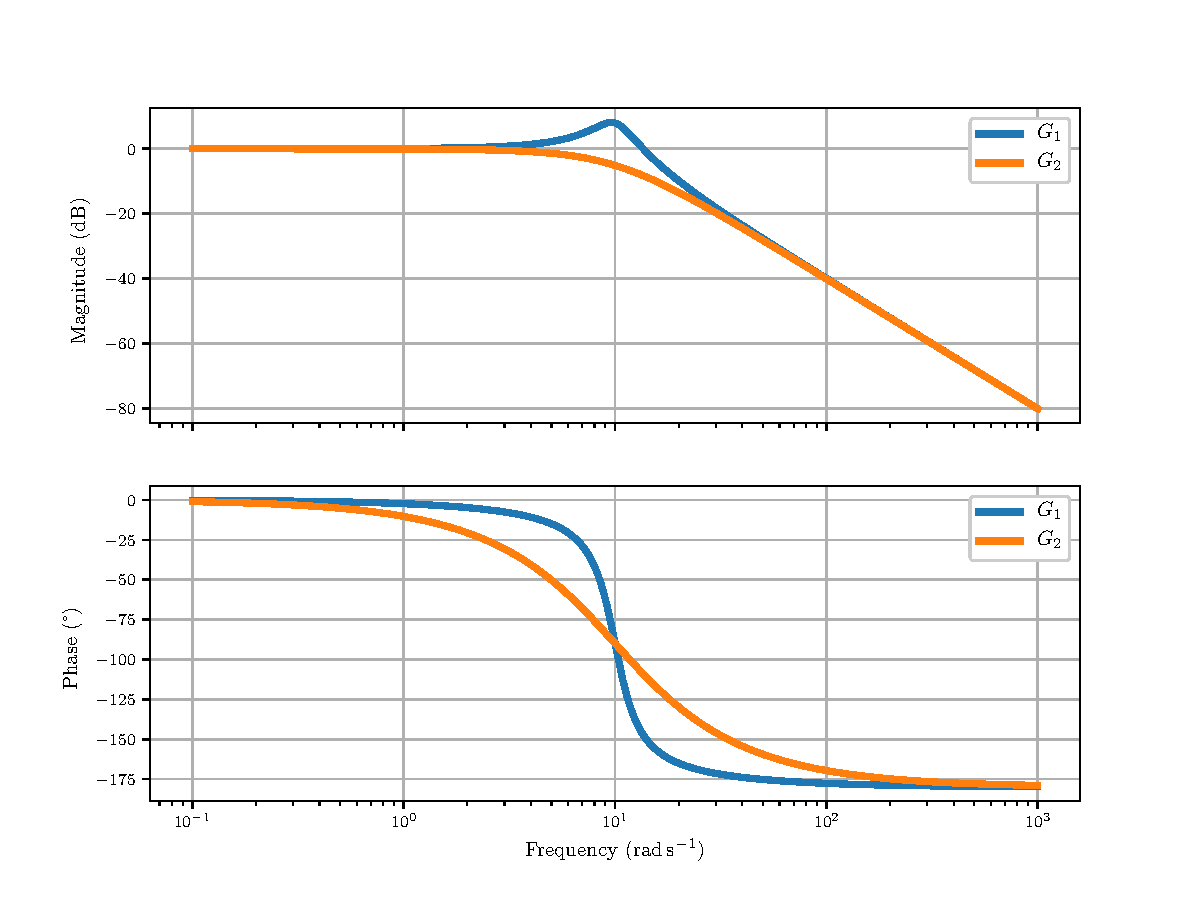
\includegraphics[width=\textwidth, height=0.6\textheight, keepaspectratio]{figures/prob1_bode.pdf}
    \caption{Frequency Response~\label{fig:prob1_bode}}
\end{figure}  

\begin{enumerate}
    \item Which of the following statements are true about the damping ratios of the two systems?
    \begin{enumerate}
        \item The damping coefficients are the same.
        \item The damping coefficient of \(G_1\) is greater than the damping coefficient of \(G_2\).
        \item The damping coefficient of \(G_2\) is greater than the damping coefficient of \(G_1\).
        \item Not enough information to make any statements about the damping ratio.
    \end{enumerate} 
    \item Which of the following statements are true about the general form of \(G_1\)?
    \begin{enumerate}
        \item It is a first order system.
        \item It must have two free \(s\) terms in the denominator since the phase ends at \SI{180}{\degree}.
        \item It must have two free \(s\) terms in the numerator since the final magnitude slope is \SI{40}{\decibel} per decade.
        \item None of the above.
    \end{enumerate}
\end{enumerate}
\clearpage

\section{Problem}\label{prob:tf_match}

The transfer functions of three systems are given as follows:
\begin{align*}
    G_1 = \frac{1}{s^2 + 0.2 s+ 1}, \qquad G_2 = \frac{2s +4}{s^2 + 0.5 s + 4}, \qquad G_3 = \frac{-2s + 4}{s^2 + 0.5 s +4}.
\end{align*}

You should accomplish the following tasks:
\begin{enumerate}
    \item Match each Bode plot shown in~\cref{fig:bode_match}  with the appropriate transfer function by indicating on each plot the correct transfer function ( i.e. \(G_1\), \(G_2\), or \(G_3\)).
        Explain the reasoning that lead to your solution.
    \item Match each response plot shown in~\cref{fig:sinusoidal_match} with the correct transfer function by indicating on each plot the correct transfer function. 
        Explain the reasoning for your solution.
        \textbf{Note:~\cref{fig:bode_match,fig:sinusoidal_match} are not in the same order.}
\end{enumerate}
\clearpage
\begin{figure}[h]
    \centering
    \begin{subfigure}{0.5\textwidth}
        \centering
        \begin{subfigure}[htbp]{\textwidth} 
            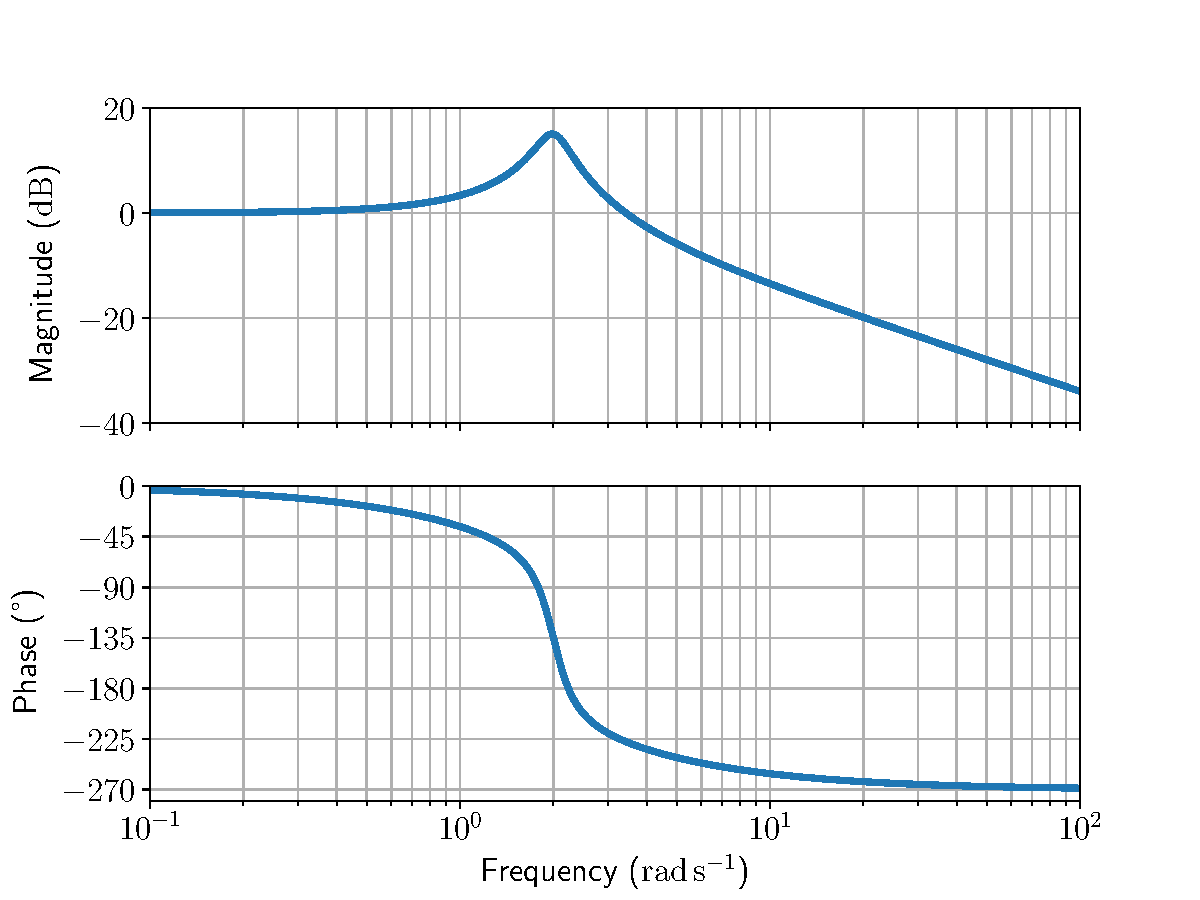
\includegraphics[width=\textwidth]{figures/G3_bode.pdf} 
        \end{subfigure}\\
        \begin{subfigure}[htbp]{\textwidth} 
            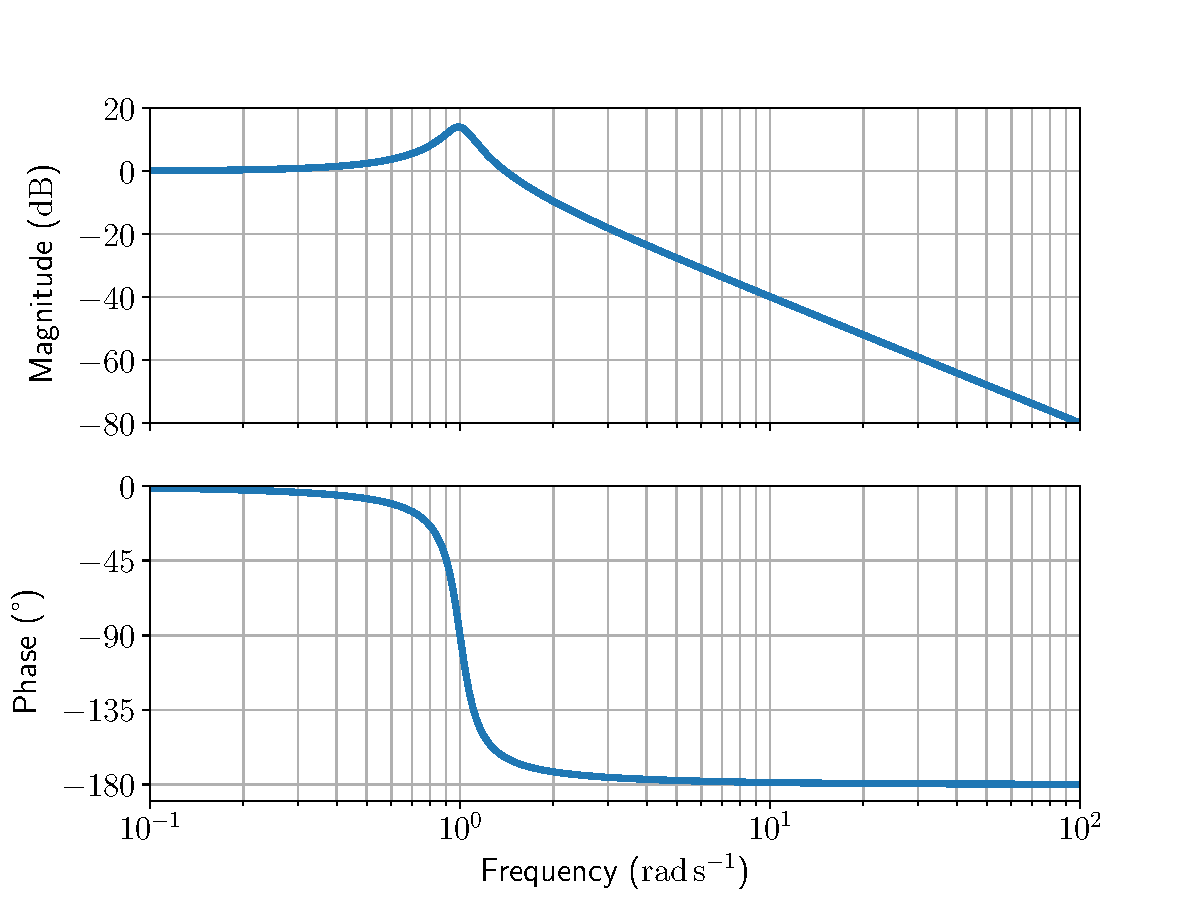
\includegraphics[width=\textwidth]{figures/G1_bode.pdf} 
        \end{subfigure} \\
        \begin{subfigure}[htbp]{\textwidth} 
            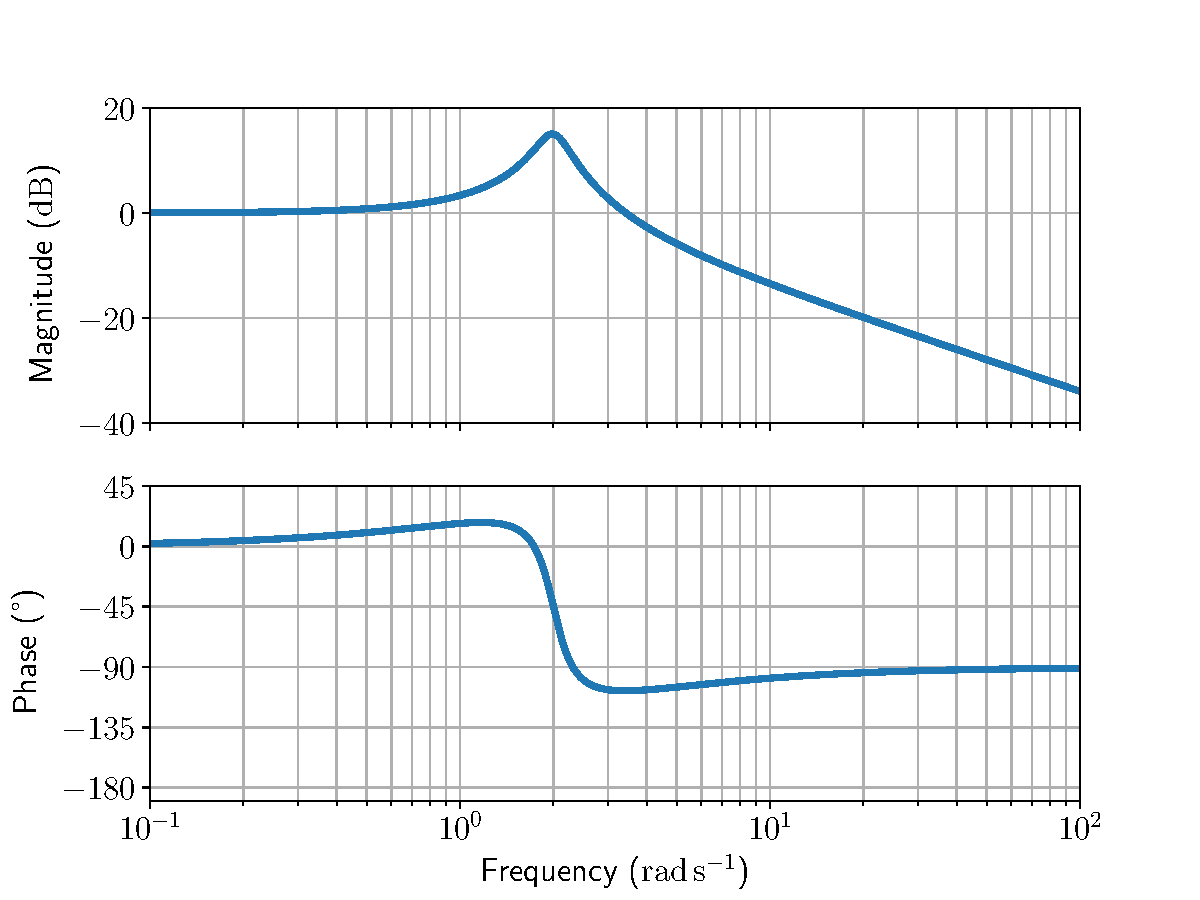
\includegraphics[width=\textwidth]{figures/G2_bode.pdf} 
        \end{subfigure} 
        \caption{Bode Plots}~\label{fig:bode_match}
    \end{subfigure}~\hfill
    \begin{subfigure}{0.5\textwidth}
        \centering
        \begin{subfigure}[htbp]{\textwidth} 
            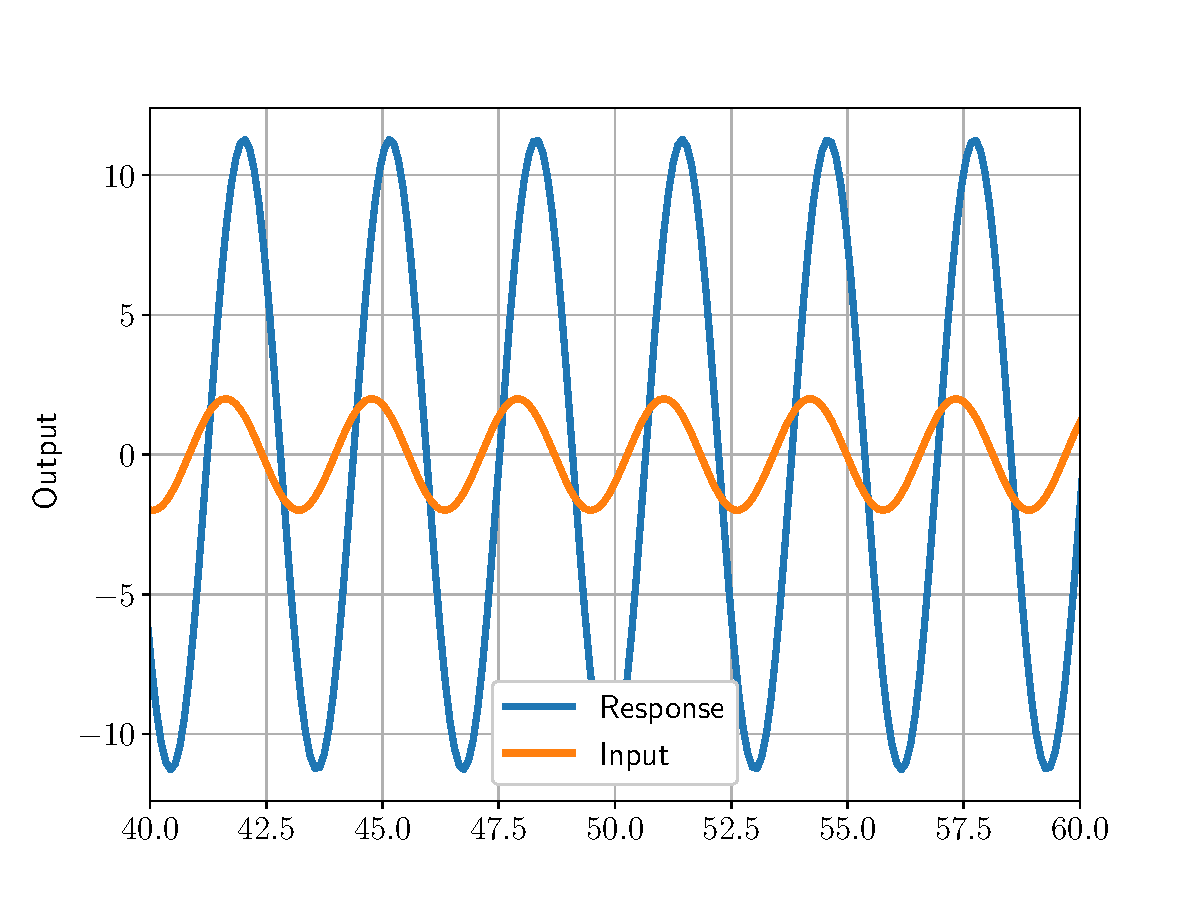
\includegraphics[width=\textwidth]{figures/G2_sinusoidal.pdf} 
        \end{subfigure}\\
        \begin{subfigure}[htbp]{\textwidth} 
            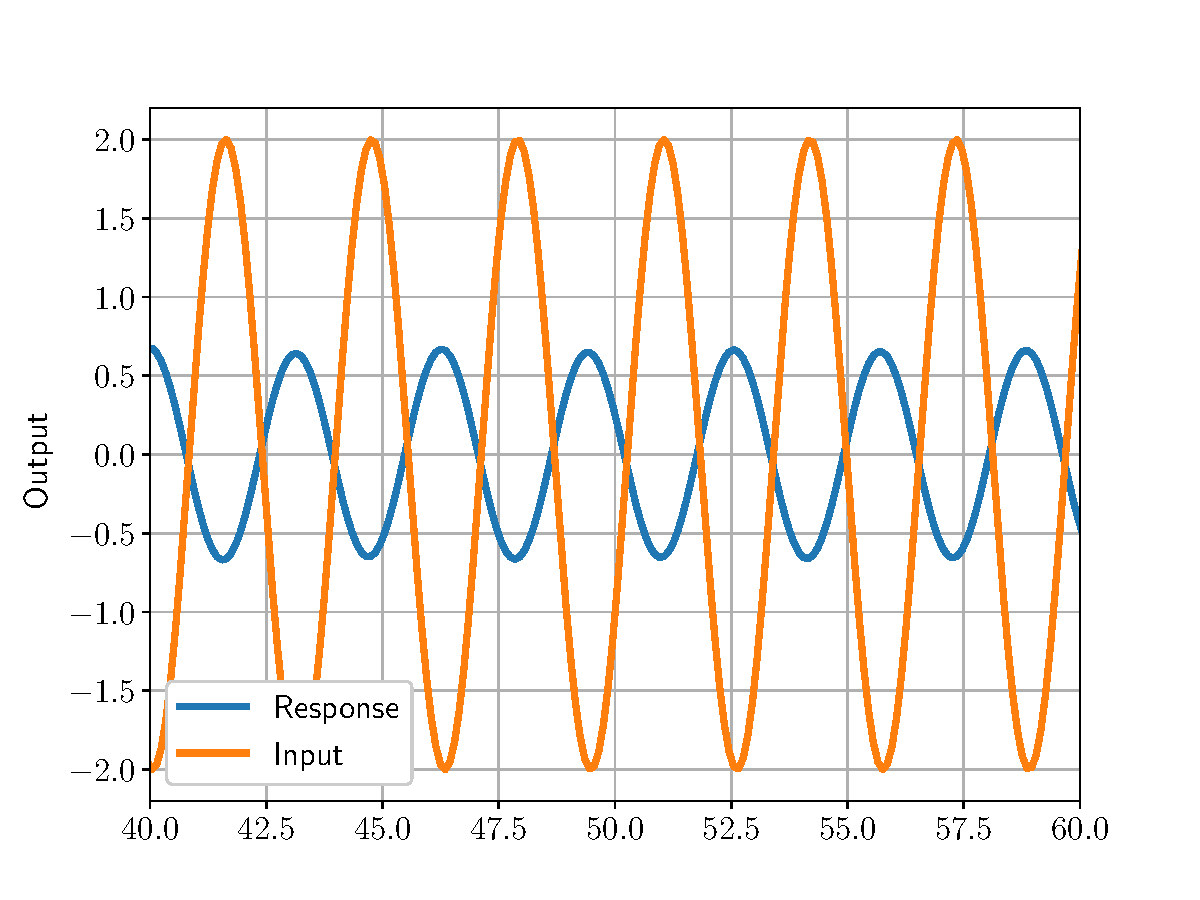
\includegraphics[width=\textwidth]{figures/G1_sinusoidal.pdf} 
        \end{subfigure} \\
        \begin{subfigure}[htbp]{\textwidth} 
            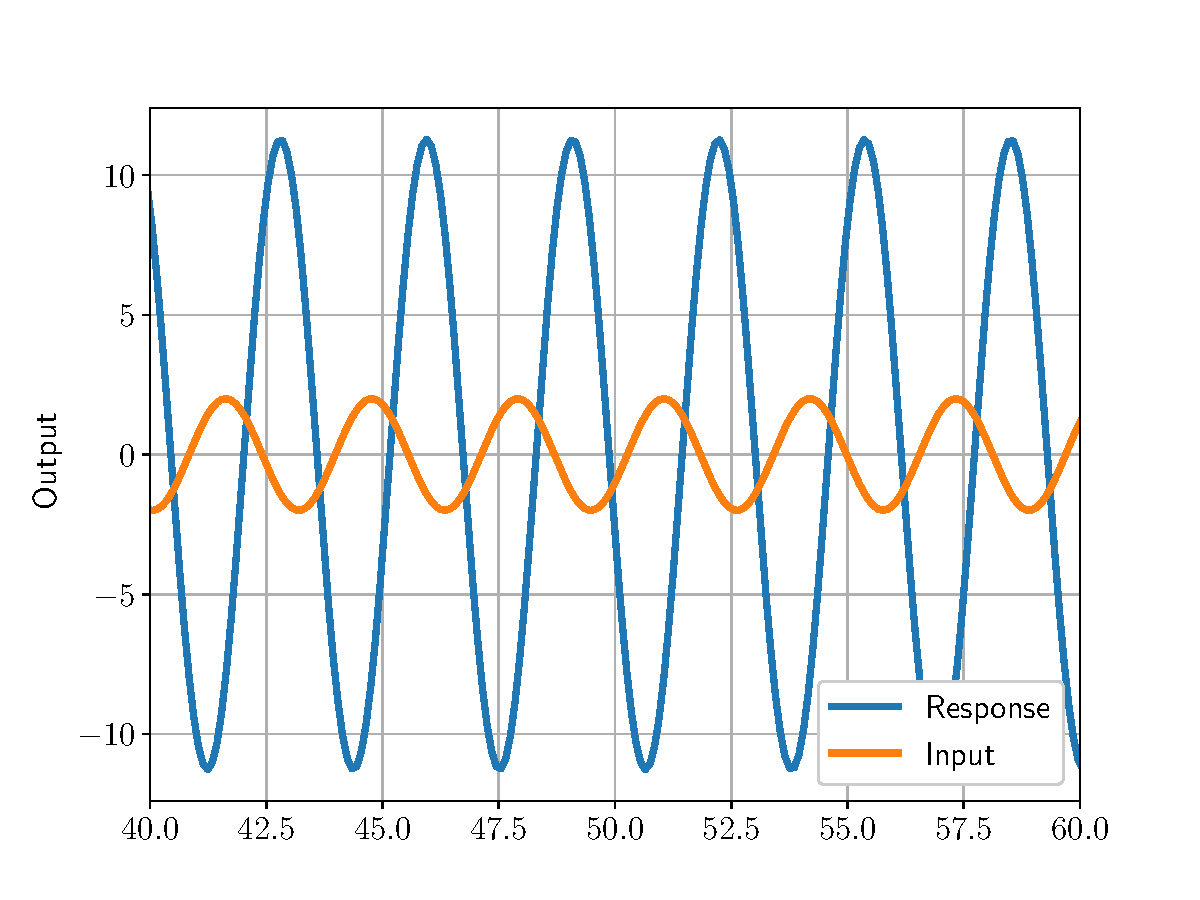
\includegraphics[width=\textwidth]{figures/G3_response.pdf} 
        \end{subfigure} 
        \caption{Sinusoidal Response}~\label{fig:sinusoidal_match}
    \end{subfigure}
    \caption{\Cref{prob:tf_match} Bode and Sinusoidal Responses}
\end{figure}
\clearpage
\section{Problem}

A transfer function is defined as
\begin{align*}
    G(s) = \frac{500 (s + 40)}{s^2 + 8s + 25}.
\end{align*}
Draw the asymptotic Bode plots for this system.

\begin{figure*}[htbp] 
    \centering 
    \begin{subfigure}[htbp]{\textwidth} 
    
\begin{tikzpicture}[]
        \begin{semilogxaxis}[
            xmin=1e0, xmax=1e4,
            ymin=0, ymax=10,
            grid=both,
            grid style={line width=0.1pt, draw=gray!65},
            major grid style={line width=0.2pt, draw=gray!95},
            yticklabels={,,},
            xticklabels={,,},
            minor tick num=4,
            width=\textwidth,
            height=0.43\textheight
        ]
        \end{semilogxaxis}
    \end{tikzpicture}
    \vspace*{0.2cm}
    \end{subfigure}

    \begin{subfigure}[htbp]{\textwidth} 
    
\begin{tikzpicture}[]
        \begin{semilogxaxis}[
            xmin=1e0, xmax=1e4,
            ymin=0, ymax=10,
            grid=both,
            grid style={line width=0.1pt, draw=gray!65},
            major grid style={line width=0.2pt, draw=gray!95},
            yticklabels={,,},
            xticklabels={,,},
            minor tick num=4,
            width=\textwidth,
            height=0.43\textheight
        ]
        \end{semilogxaxis}
    \end{tikzpicture}
    \end{subfigure}
\end{figure*}
\clearpage
\newpage
\mbox{}
\clearpage
\section{Problem}
Consider the electrical circuit shown in~\cref{fig:elec_circuit}:
\begin{enumerate}
    \item Find the differential equations which govern the behavior of the electrical system.
    \item Construct the state space representation of the system. 
        Assume the desired output is the charge in the system.
    \item Find the output response of the system assuming zero initial conditions and a step input of \(u(t) = \SI{24}{\volt}\)
\end{enumerate}
\begin{figure}[htbp]
\centering
\begin{scaletikzpicturetowidth}{0.5\textwidth}
    \begin{tikzpicture}[scale=\tikzscale]
        \draw (0,0) to[american voltage source,v<=\( u(t)\)] (0,2) 
        to[inductor, l^=1<\henry>] (2,2) to[resistor, l=3<\ohm>] (2,0) 
        to[capacitor, l^=0.5<\farad>] (0,0); 
    \end{tikzpicture}
\end{scaletikzpicturetowidth}
\caption{Electrical Circuit~\label{fig:elec_circuit}}
\end{figure}
\clearpage
\newpage
\thispagestyle{plain}
\mbox{}
\clearpage
\section{Problem}

For the electrical system in~\cref{fig:elec_circuit_2}:
\begin{enumerate}
    \item Find the differential equations for the system.
    \item Find the state space representation of the system with your state vector defined as
        \begin{align*}
        \vb{x} = \begin{bmatrix}q_1 & i_1 & q_2 & i_2\end{bmatrix}^T,
        \end{align*}
        where \(q_1, i_1\) represent the charge and current in the left loop while \(q_2, i_2\) represent the charge and current in the right loop. 
        The output is defined as
        \begin{align*}
        y = \begin{bmatrix} q_1 & q_2 \end{bmatrix}^T.
        \end{align*}
\end{enumerate}
\begin{figure}[htbp]
\centering
\begin{scaletikzpicturetowidth}{0.8\textwidth}
    \begin{tikzpicture}[scale=\tikzscale]
        \draw (0,0) to[american voltage source,v<=\( u(t)\)] (0,2) 
        to[resistor, l^=$R_1$] (2,2) to[resistor, l=$R_2$] (2,0) 
        to[capacitor, l^=$C$] (0,0); 
        \draw (2,2) to[short] (4,2)
        to[inductor, l=$L$] (4,0) to[short] (2,0);
    \end{tikzpicture}
\end{scaletikzpicturetowidth}
\caption{Electrical Circuit~\label{fig:elec_circuit_2}}
\end{figure}
\clearpage
\newpage
\mbox{}
\clearpage
\section{Problem}
Given the state space representation is defined as
\begin{align*}
    \vb{\dot{x}} &= A \vb{x} + B \vb{u}, \\
    \vb{y} &= C \vb{x} + D\vb{u},
\end{align*}
\textbf{DERIVE} the expression for the transfer function \(\frac{\vb{Y}(x)}{\vb{U}(s)}\).
\vspace{13cm}
\section{Problem}

List at least two advantages of state-space or ``modern control'' techniques as compared to ``classical control'' approaches.
\vspace{5cm}
\clearpage
\end{document}  
